\documentclass[11pt]{article}

\newcommand{\cnum}{CS188}
\newcommand{\ced}{Winter 2017}
\newcommand{\ctitle}[3]{\title{\vspace{-0.5in}\cnum, \ced\\Problem Set #1: #2\\Due #3}}
\usepackage{enumitem}
\usepackage{amsmath}
\usepackage{graphicx}
\graphicspath{ {images/} }

\newcommand{\solution}[1]{{{\color{blue}{\bf Solution:} {#1}}}}
\usepackage[usenames,dvipsnames,svgnames,table,hyperref]{xcolor}

\renewcommand*{\theenumi}{\alph{enumi}}
\renewcommand*\labelenumi{(\theenumi)}
\renewcommand*{\theenumii}{\roman{enumii}}
\renewcommand*\labelenumii{\theenumii.}


\begin{document}
\ctitle{0}{Math Prerequisites}{Jan 19,2017}
\author{Rohan Varma}
\date{}
\maketitle
\vspace{-0.75in}

\section{Problem 1}
\begin{enumerate}
\item 

\solution{
\[
\displaystyle \frac{\partial y}{\partial x} = -x e^{-x}\sin{z} + \sin{z}e^{-x} = e^{-x}\sin{z}(1 - x)
\]
}

\vspace{10cm}
\end{enumerate}

\newpage
\section{Problem 2}

\solution{Solution to problem 2}
\begin{enumerate}
\item Problem 2a

\solution{
y^{T}z = 1*2 + 3*3 = 11
}

\vspace{2cm}
\item Problem 2b

\solution{
\[
   \begin{bmatrix}
    2 & 4  \\
    1 & 3 
  \end{bmatrix} * \begin{bmatrix} 1 & \\ 3 \end{bmatrix}
 = 1 * \begin{bmatrix} 2 & \\ 1 \end{bmatrix} + 3 * \begin{bmatrix} 4 & \\ 3 \end{bmatrix} = \begin{bmatrix} 14 & \\ 10 \end{bmatrix}
\]  
}

\vspace{2cm}
\item Problem 2c

\solution{
\bold{X} is invertible since the two vectors given by its columns are linearly independent. The inverse can be calculated with the well-known formula for the inverse of a 2 x 2 invertible matrix:  \newline
\[X^{-1} = \frac{1}{ad-bc} * \begin{bmatrix} d & -b \\ -c & a \end{bmatrix} = \frac{1}{2} * \begin{bmatrix} 3 & -4 \\ -1 & 2 \end{bmatrix}
\]
}

\vspace{2cm}
\item Problem 2d

\solution{
The rank is the number of leading ones in reduced-row echelon form. Equivalently, it is the number of linearly independent rows (or columns) in the matrix, which is 2 as stated above. So rank(X) = 2.
}

\end{enumerate}
\newpage

\section{Problem 3}

\solution{Solution to problem 3}
\begin{enumerate}
\item Problem 3a

\solution{
\mu_{sample} = \[\frac{1}{N} \sum_{i = 1}^{N} x_{i} = \frac{1 + 1 + 0 + 1 + 0}{5} = 0.6  \]
}

\vspace{0.5cm}
\item Problem 3b

\solution{
\sigma^{2}_{sample} = \[\frac{1}{N-1} \sum_{i = 1}^{N} ){x_i - \mu_{sample}}) = 0.3
}

\vspace{0.5cm}
\item Problem 3c

\solution{
Since each particular sample is independent of the other, we have \[P = P(1) * P(1) * P(0) * P(1) * P(0) = \frac{1}{2^{5}} = \frac{1}{32} \]
}

\vspace{0.5cm}
\item Problem 3d

\solution{
Let P(S) denote the probability of sample S. Let p = P(X = 1). Then, one has: \newline \[P(S) = p^{3}(1-p)^{2} \]. \newline We want to find p such that the function is maximized (and p is in between 0 and 1 otherwise P(S) = 0), so we take the derivative and set it equal to zero: 
\newline
\[\frac{\partial{P(S)}}{\partial{p}} = 5p^{4} - 8p^{3} + 3p^{2} = 0 \] 
 \[ 5p^{2} - 8p +3 = 0 \] Solving for p, we obtain \[p =  \frac{3}{5} \]

}

\vspace{0.5cm}
\item Problem 3e

\solution{
\[ P(X=T|Y=b) = \frac{P(X=T,Y=b)}{P(Y=b)} = \frac{.1}{.25} = 0.4 \]
}

\end{enumerate}
\newpage
\section{Problem 4}

\solution{Solution to problem 4}
\begin{enumerate}
\item Problem 4a

\solution{
False.
}

\vspace{0.5cm}
\item Problem 4b

\solution{
True.
}

\vspace{0.5cm}
\item Problem 4c

\solution{
False.
}

\vspace{0.5cm}
\item Problem 4d

\solution{
False
}

\vspace{0.5cm}
\item Problem 4e

\solution{
True.
}




\end{enumerate}
\newpage

\section{Problem 5}

\solution{Solution to problem 5}
\begin{enumerate}
\item Problem 5a

\solution{
v
}

\vspace{0.5cm}
\item Problem 5b

\solution{
iv
}

\vspace{0.5cm}
\item Problem 5c

\solution{
ii
}

\vspace{0.5cm}
\item Problem 5d

\solution{
i
}

\vspace{0.5cm}
\item Problem 5e

\solution{
iii
}

\end{enumerate}

\newpage

\section{Problem 6}

\solution{Solution to problem 6}
\begin{enumerate}
\item Problem 6a

\solution{
\[mean:  p \]
\[ variance: p(1-p) \]
}

\vspace{0.5cm}
\item Problem 6b

\solution{
\[ Var[X] = E[(X - E[X])^{2} ] = \sigma^{2} \]
For 2X, We know that
\[ E[2X] = 2E[X] \]
So by substitution
\[ Var[2X] = E[(2X - 2E[2X])^{2} ] = 4E[(X - E[X])^{2}] = 4\sigma^{2}\] 
which is the variance of 2X. This makes sense since the spread of the data becomes twice the original, increasing the standard deviation by 2, and the variance is the standard deviation's square.
\newline \newline
For X + 2, we know that
\[E[X + 2] = E[X] + E[2] = E[X] + 2 \]
Therefore, 
\[ Var[X + 2] = E[(X + 2 - E[X + 2])^{2}] = E[(X + 2 - E[X] - 2)^{2}] = E[(X - E[X])^{2}] = \sigma^{2} \]
so the variance does not change if we add 2. This makes sense since the overall spread of the data is the same
}

\end{enumerate}
\newpage

\section{Problem 7}

\solution{Solution to problem 7}
\begin{enumerate}
\item Problem 7a

\solution{
i. Both. The functions differ by a constant, so their asymptotic growth rate is the same. \[ f(n) = \Theta(g(n)) \]
ii. \[g(n) = O(f(n)) \]. An exponential function grows asymptotically faster than a polynomial function.
\newline
iii. \[g(n) = O(f(n)) \]. f(n) grows asymptotically faster than g(n). This can be seen by taking the limit as n becomes large:
\[\lim_{n\to\infty} \frac{f(n)}{g(n)} = \lim_{n\to\infty} (\frac{3}{2})^n = \infty \]
}

\vspace{0.05cm}
\item Problem 7b

\solution{\newline
find-transition-index(arr, i, j): \newline
    if i is greater or equal to j, return -1 (no index found) \newline
    let mid = i + floor( (j-i)/2) \newline
    if arr[mid] == 0 and arr[mid + 1] == 1: return mid \newline
    if arr[mid] == 0 and arr[mid + 1] == 0: return find-transition-index(arr, mid+1, j) \newline
    else return find-transition-index(arr,i,mid)
    \newline
    \newline
    The algorithm is correct since it picks the middle index at each step, and sees if there is a transition. If not, half the problem space can be discarded based on the values of arr[mid] and arr[mid+1], and it recursively searches the correct half until a transition is found or i exceeds j, implying no transition exists.
    \newline
    \newline
    Looking at the algorithm, we see that the problem size reduces by half each time find-transition-index is called. Therefore, we have the following recurrence: 
    \[ T(n) = T(n/2) + O(1) \] with O(1) base cases. This recurrence solves to O(n log n).
    
}


\end{enumerate}
\newpage

\section{Problem 8}

\solution{Solution to problem 8}
\begin{enumerate}
\item Problem 8a

\solution{
\[ E[XY] = \sum_{i =1}^{N} x_{i}y_{i}p(x_i,y_i) \] By the product rule, \[ p(x_i, y_i) = p(x_i | y_i)p(y) \] but since x, y are independent, \[p(x_i | y_i) = p(x_i) \] Therefore, \[p(x_i, y_i) = p(x_i)p(y_i)\] and \[E[XY] = \sum_{i = 1}^{N} x_{i}p(x_i)y_{i}p(y_i) = \sum_{i = 1}^{N} x_{i}p(x_i)} * \sum_{i = 1}^{N}y_{i}p(y_{i}) = E[X]*E[Y] \]
}

\vspace{0.5cm}
\item Problem 8b

\solution{\newline
i. Assuming a fair die, by the law of large numbers, the number of times a 3 shows up should be close to 1000. 
\newline 
ii. The central limit theorem says that the distribution of X converges weakly to the Gaussian as n tends to infinity.
}

\end{enumerate}
\newpage

\section{Problem 9}

\solution{Solution to problem 9}
\begin{enumerate}
\item Problem 9a

\includegraphics[scale=0.5]{vec.png}

\vspace{0.5cm}
\item Problem 9b

\solution{
i. An eigenvalue is a scalar lambda such that \[ A(v) = \lambda v \] where A is a square matrix and v is a vector. \newline An eigenvector is a (nonzero) vector v who's direction does not change when the linear transformation A is applied to it. In other words, v is an eigenvector of a square matrix A if the product A*v is a scalar multiple of v. \newline 

ii. \[A = \begin{bmatrix}
    2 & 1  \\
    1 & 2 
  \end{bmatrix} \]
  \[det(A - \lambda I) = det( \begin{bmatrix} 2 - \lambda & 1 \\ 1 & 2 - \lambda \end{bmatrix}) = (2-\lambda )^{2} -1 = 0
 \]
 \[ \lambda_1 = 3 , \lambda_2 = 1 \]
 For the corresponding eigenvector $v_1$ of $\lambda_1 $, we want to find a vector in the nullspace of $ A - 3I $:
 \[ A - 3I = \begin{bmatrix} -1 & 1 \\ 1 & -1 \end{bmatrix} \]
 \[\begin{bmatrix} -1 & 1 \\ 1 & -1 \end{bmatrix} * v_1 = 0 \]
 \[v_1 = \begin{bmatrix} 1 \\ 1 \end{bmatrix} \]
 For the corresponding eigenvector $v_2$ of $\lambda_2 $, we want to find a vector in the nullspace of $ A - I $: 
 \[ A - I = \begin{bmatrix} 1 & 1 \\ 1 & 1 \end{bmatrix} \]
 \[ \begin{bmatrix} 1 & 1 \\ 1 & 1 \end{bmatrix} * v_2 = 0 \] \[v_2 = \begin{bmatrix} -1 \\ 1 \end{bmatrix} \]
 iii. We show this by induction: \newline
 Base Case: k = 1: we have $ Av = \lambda v $ for n eigenvalues and n eigenvectors. This is given. \newline
 Inductive Hypothesis: Assume the n eigenvalues of $ A^{k-1} $ take the form $ \lambda^{k-1} $. That is, assume that there are n distinct eigenvalues and eigenvectors that satisfy $ A^{k-1}v  = \lambda^{k-1}v $ \newline Inductive Step: We show that the hypothesis holds for j = k, namely, that the eigenvalues of $A^k$ fulfill $A^{k}v = \lambda^{k}v $ where $\lambda$ and $v$ represent the n eigenvalues and eigenvectors of $A$. First, we notice
 \[ A^{k}v = AA^{k-1}v\]
 From the inductive hypothesis, we know \[A^{k-1}v = \lambda^{k-1}v \]
 Therefore,
 \[ A^{k}v = A\lambda^{k-1}v = \lambda^{k-1}Av \]
 Since $ Av = \lambda v $, 
 \[A^{k} v = \lambda^{k-1}\lambda v = \lambda^{k} v \]
 Showing what we wanted. Since we showed this for any eigenvalue corresponding to its eigenvector, it applies for all n eigenvalues and eigenvectors of $ A $. 
}

\vspace{0.5cm}
\item Problem 9c

\solution{ \newline
i. \[\frac{\partial{(a^{T}x)}}{\partial{x}} = a^{T} \]
ii. \[ \frac{\partial{(x^{T}Ax)}}{\partial{x}} = A^{T}x + x^{T}A \]
\[ \frac{\partial^2{(x^{T}Ax)}}{\partial{x^2}} = \frac{\partial{(A^Tx + x^TA)}}{\partial{x}} = A^{T} + A = 2A \]
}
\vspace{0.5cm}
\item Problem 9d
\solution{ \newline
i. Consider two points, $x_1$ and $x_2$ on the line. This implies that \[ w^Tx_1 + b = w^Tx_2 + b = 0 \] \[w^Tx_1=w^Tx_2\]
\[w^T(x_1-x_2) = 0 \]
We notice that the vector given by $v = x_1$ - $x_2$ is a vector parallel to our line. Since the dot product of $w^T$ and a vector $v = x_1 - x_2 $ is zero, the vector $w$ must be orthogonal to $v$, implying that $w$ is orthogonal to $w^Tx + b = 0$.
\newline \newline
ii. First, we let x* be the point on the line that is closest to the origin. Then, one has $ x* = min a^{T}a $ given the constraint $ w^{T}a + b = 0 $. Taking the derivative and using Lagrange multipliers, one obtains: \[2x* = \lambda w \longrightarrow  x* = \frac{\lambda}{2}w \]
Plugging the value in the constraint, we have \[ w^{T}a + b = 0 \] \[w^{T}(\frac{\lambda}{2}w) +b =  0 \] \[\lambda = \frac{-2b}{w^Tw} \] \[x* = \frac{-bw}{w^tw} \]
Having calculate $ x* $, we can now calculate its distance from the origin: \[d = \sqrt{(x*)^{T}x*} = \sqrt{(\frac{-b}{w^Tw})^2 w^Tw} = \frac{b}{w^Tw}\sqrt{w^Tw} = \frac{b}{||w||} \] as expected.
}

\newpage

\section{Problem 10}

\solution{Solution to problem 10}
\begin{enumerate}
\item Problem 10a

\solution{
}
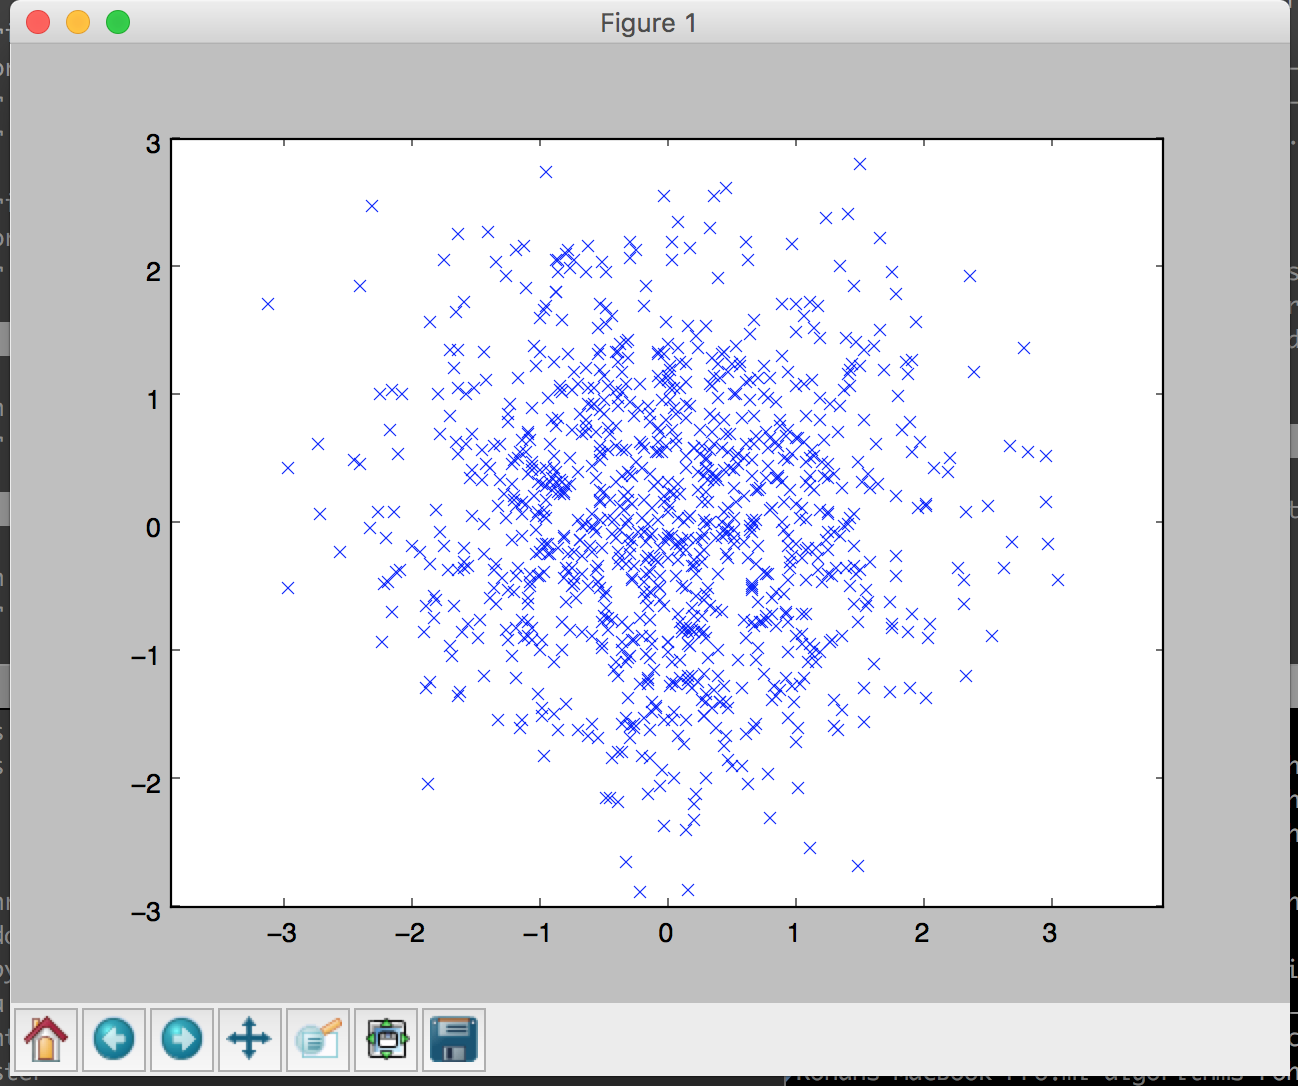
\includegraphics[scale=0.40]{fig1.png}
\vspace{0.5cm}
\item Problem 10b

\solution{
The distribution is centered around 1, not zero.
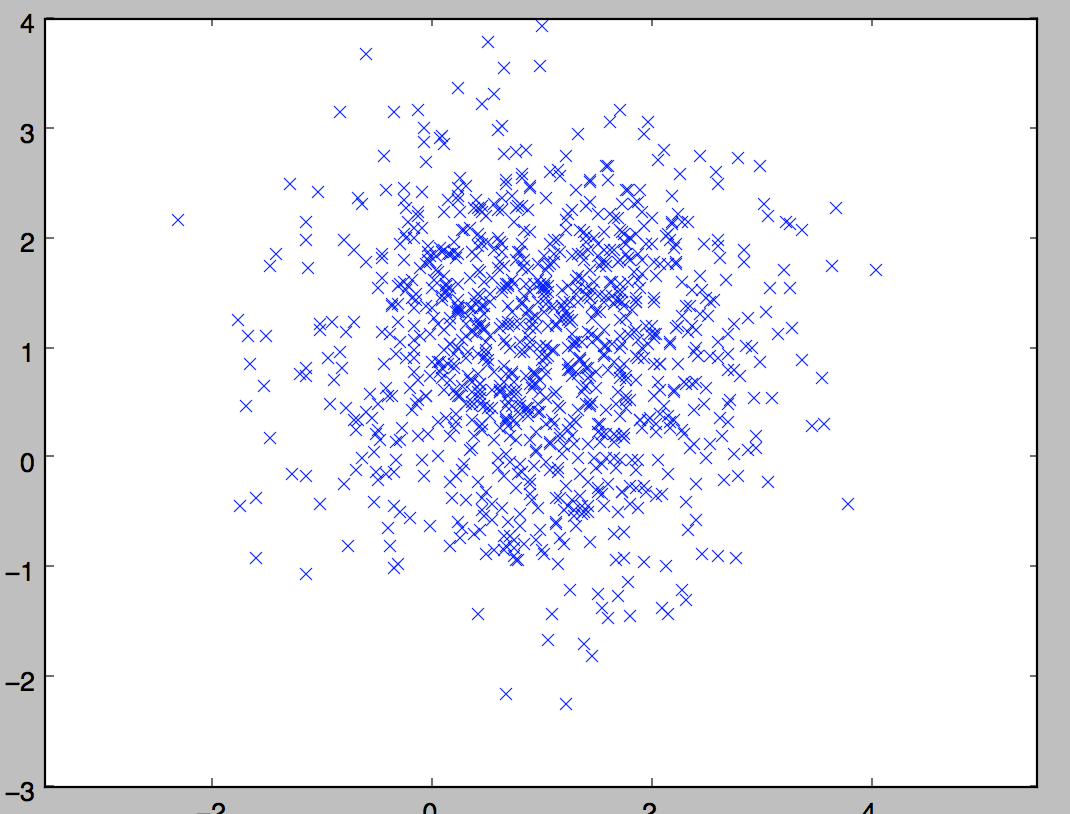
\includegraphics[scale=0.40]{fig2.png}
}

\vspace{0.5cm}
\item Problem 10c

\solution{
The data becomes more spread out. \newline
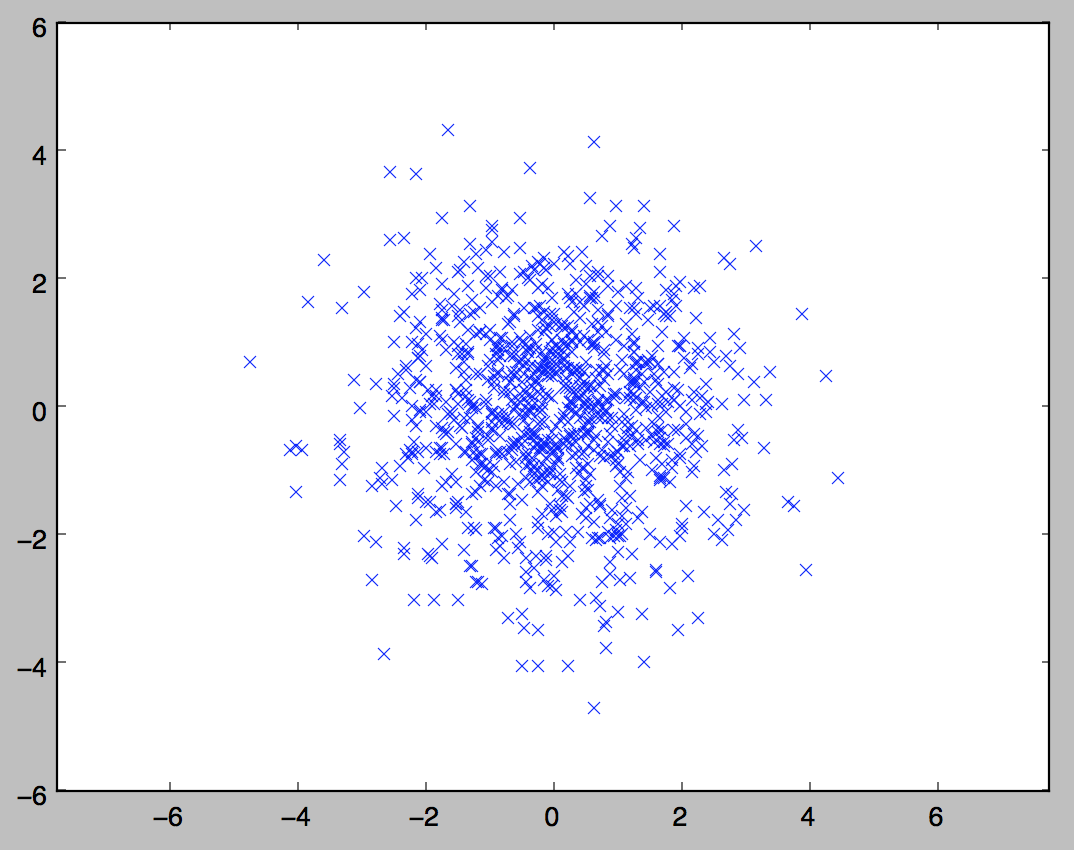
\includegraphics[scale = 0.40]{fig3.png}
}

\vspace{0.5cm}
\item Problem 10d

\solution{
The data become skewed, stretching from the lower left to the upper right. \newline
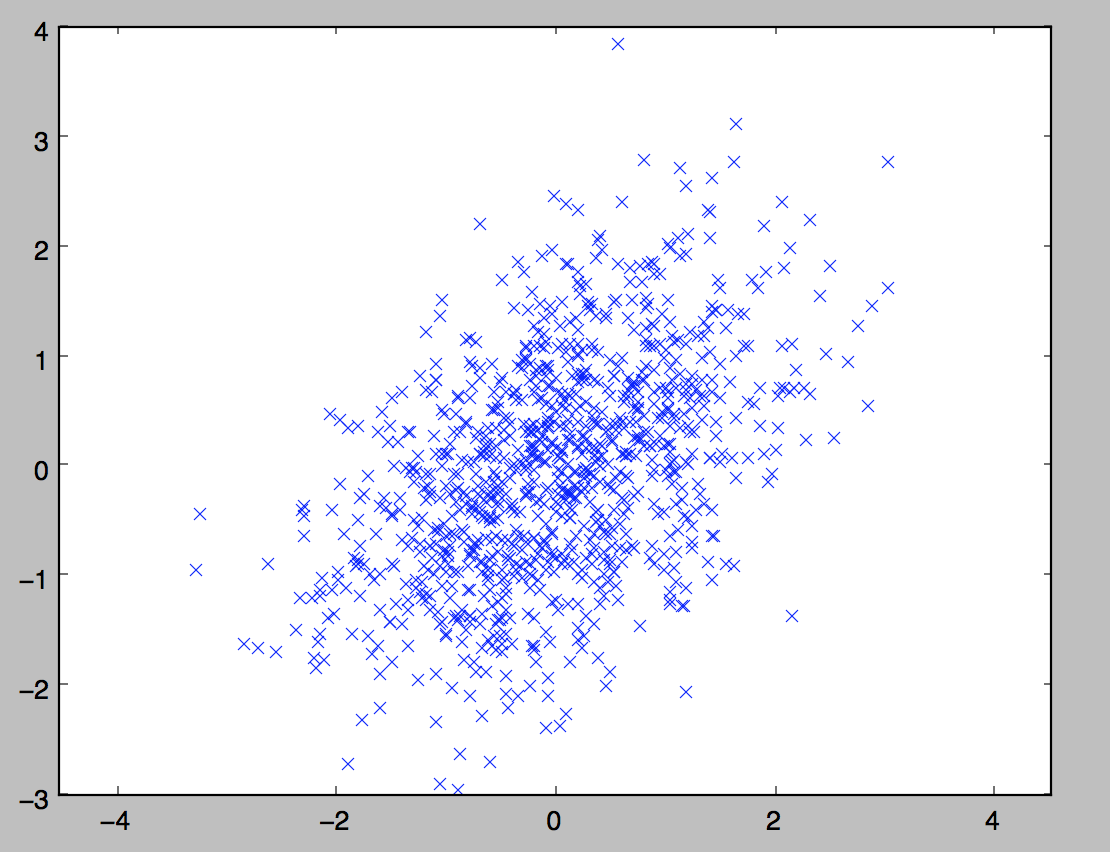
\includegraphics[scale=0.40]{fig4.png}
}

\vspace{0.5cm}
\item Problem 10e

\solution{
The data become skewed so that it stretches from the upper left to the bottom right.  \newline
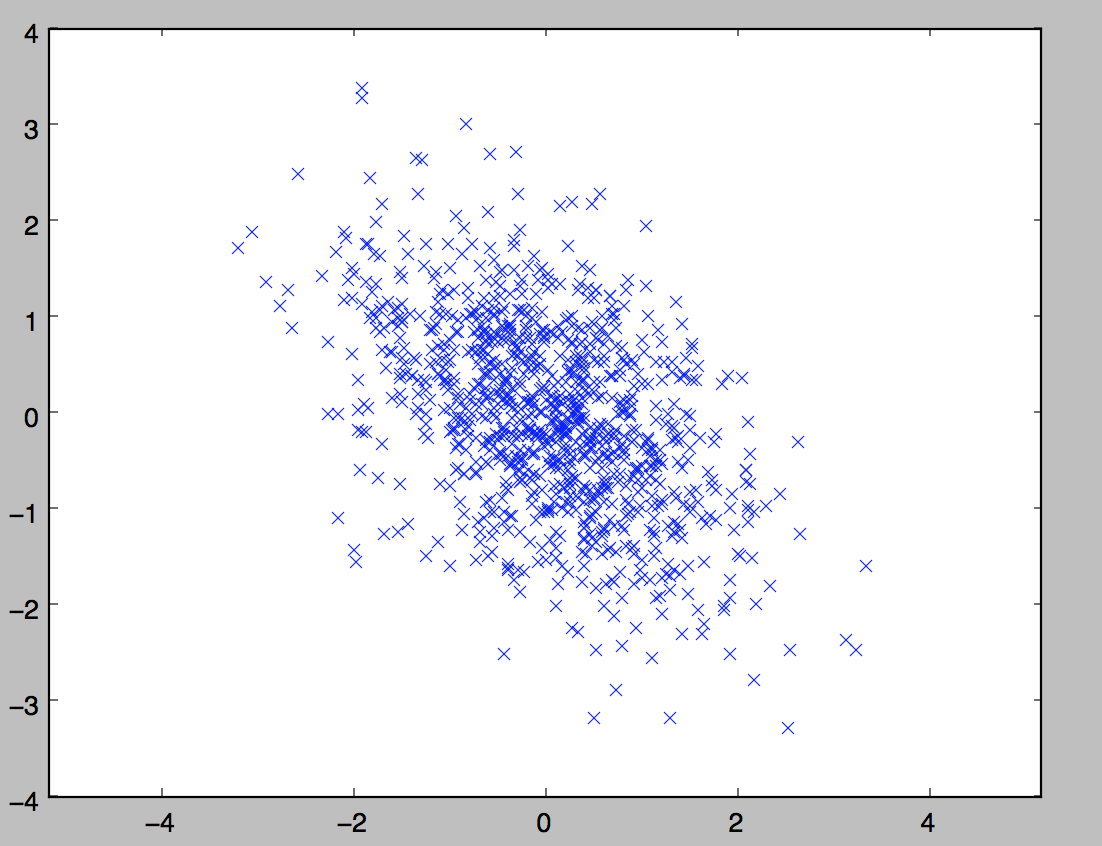
\includegraphics[scale=0.5]{fig5.png}
}

\end{enumerate}



\end{enumerate}
\newpage

\section{Problem 11}

\solution{Solution to problem 11}
\begin{enumerate}
\item Problem 11

\solution{
\[A = \begin{bmatrix} 1 & 0 \\ 1 & 3 \end{bmatrix} \]
\[det(A - \lambda I) = det(\begin{bmatrix} 1 - \lambda & 0 \\ 1  & 3 - \lambda \end{bmatrix}) = (1-\lambda)(3-\lambda), \lambda_{largest} = 3  \]
Find a vector v in the nullspace of A - 3I:
\[(A - 3I)v = \begin{bmatrix} -2 & 0 \\ 1 & 0 \end{bmatrix}(v) = 0 \]
\[v = \begin{bmatrix} 0 \\ 1 \end{bmatrix} \]
}

\end{enumerate}

\newpage

\section{Problem 12}

\solution{Solution to problem 12}
\begin{enumerate}
\item Problem 12a

\solution{
Name: The MNIST Database of Handwritten Digits
}

\vspace{0.5cm}
\item Problem 12b

\solution{
Data set is available at http://yann.lecun.com/exdb/mnist/
}

\vspace{0.5cm}
\item Problem 12c

\solution{
The dataset contains images of handwritten data as well as labels that tell us which number the handwritten digit corresponds to. Each training example is a pair (image, label) and the features of this training set are the individual pixels in the image, and we wish to predict the number that the image represents.
}

\vspace{0.5cm}
\item Problem 12d

\solution{
There are 60,000 training examples in the dataset (ie, 60,000 (image, label) pairs) as well as a testing set of 10,000 examples that can be used to evaluate your model after it is trained. 
}

\vspace{0.5cm}
\item Problem 12e

\solution{
Each training example contains a 28 x 28 black and white image. Therefore, there are $ 28^2 = 784$ features for each training example, where each feature is either 0 or 1, representing the pixel at that position. Even though the image is a square, when a model sees the features, they are generally flattened out to a 784 dimensional vector. We are then left with a 784 dimensional vector of numbers which we can feed through models (artificial neural networks for example) to find a function that maps images to numbers. 
}





\end{enumerate}


\end{document}
